\documentclass[dvipdfmx]{jsarticle}
\usepackage[T1]{fontenc}
\usepackage[dvipdfmx]{hyperref}
\usepackage{lmodern}
\usepackage{latexsym}
\usepackage{amsfonts}
\usepackage{amssymb}
\usepackage{mathtools}
\usepackage{amsthm}
\usepackage{multirow}
\usepackage{graphicx}
\usepackage{wrapfig}
\usepackage{here}
\usepackage{float}
\usepackage{ascmac}
\usepackage{url}
\usepackage{cite}

\title{卒業研究 最終発表 詳細資料}
\author{古市研究室 2021年度生\\5419045 高林 秀}
\date{\today}

\begin{document}

\maketitle

\begin{abstract}
    本稿は、2023年度卒業研究最終発表における詳細資料である。\par
    本稿では、卒業研究(以下、本研究とする)の目的、方法、結果、考察を時間の関係で発表できなかった部分を含め詳細にまとめるものである。
\end{abstract}
\tableofcontents

\section{研究の概要}
    この章では、本研究のおおまかな概要、目的、先行研究について述べる。
    \subsection{研究概要}
        本研究では、我が国の伝統的な外遊びである「ドロケー」を、AIを使って対戦させる事を行う。本研究の目的は以下の通り。
        \begin{itemize}
            \item 研究内容 : AI(人工知能)によるドロケーにおける戦略行動の観察
            \item 研究目的
                \begin{itemize}
                    \item 各々の役割に応じて、適切な戦略行動をとることができるかを知る
                    \item AIがドロケーを遊べるようになるまでどのくらいの期間を要するか観察する
                    \item 個人レベルでの戦略だけでなく、チームとして戦略的に行動することを学習できるかを観察する。
                \end{itemize}
        \end{itemize}
    \subsection{先行研究について}
        本研究には、研究を始めるきっかけとなった先行研究がある。それに関して簡単に紹介する。\par
        先行研究として、2019年に米国の非営利AI研究機関"OpenAI"により発表された、「かくれんぼAI\cite{openAI}」が本研究を始めるきっかけである。\par
        この研究は、3Dの学習環境、鬼役のエージェント、逃走役のエージェントを用意し、AI同士でかくれんぼをさせた実験である。\par 
        最初は、お互いにランダムに動き回るだけだったが、次第に学習し独自の戦略や対処法を生み出した。環境に用意されたオブジェクトを利用し独自の戦略を学習したという結果が記録されている。
        具体的な戦略としては以下のようなものがある。
        \begin{itemize}
            \item 逃走役は環境内の移動可能なオブジェクトを使って、自身を守るシェルターを構築した。※図1
            \item 鬼役は、逃走役が構築したバリケードやシェルターを突破するために、三角形のオブジェクトを使ってバリケードを超えるなどの戦略をあみ出した。※図2
        \end{itemize}
        \begin{figure}[H]
            \begin{minipage}[b]{0.5\linewidth}
                \centering
                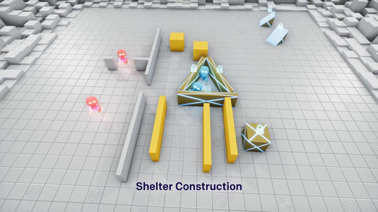
\includegraphics[scale=0.4]{images/openAI1.png}
                \caption{シェールターを構築する逃走役AI(青)}
            \end{minipage}
            \begin{minipage}[b]{0.5\linewidth}
                \centering
                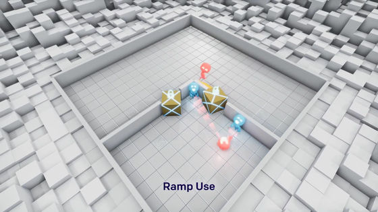
\includegraphics[scale=0.4]{images/openAI2.png}
                \caption{バリケードを突破する鬼役AI(赤)}
            \end{minipage}
        \end{figure}
        この研究では強化学習という方法に分類される機械学習を用いており、このような学習方法をとるAIに関して次のことが示された。
        \begin{itemize}
            \item 標準的な強化学習アルゴリズムが、複雑な戦略やスキルを学習させることができる。
            \item 複数エージェントを用いた方法は、非常に複雑で人間に関連した行動を導き出す可能性がある。
            \item ドアやバリケードなどの環境内に存在する物理オブジェクトをAIが自身のニーズに合わせて適切に活用することができる。
            \item 人間が解釈可能な以下の6段階の学習を示した。
            \begin{enumerate}
                \item 鬼役が逃走役を追いかけることを学び、逃走役は鬼役からに逃げることを学習
                \item 逃走役は壁などの道具の使い方を学習し、シェルターを作るようになった
                \item 鬼役はスロープを使ってジャンプし、逃走役のシェルターに飛び込むことを学習
                \item 逃走役は、スロープを隠すことを学習
                \item 鬼役は、スロープを使わずとも、固定されていない箱の上に乗り慣性でジャンプできる、Box surfing = 箱サーフィン、を学習
                \begin{itemize}
                    \item これに関しては、シミュレーターのバグをついたものである。
                \end{itemize}
                \item 逃走役は、固定されていない箱を固定することを学習する
            \end{enumerate}
        \end{itemize}
        これらの結果は、マルチエージェントの学習が、物理的に根拠のある人間に関連した行動につながることを示した。\par 
        これ以上の説明は省略するが、この研究の内容を詳細にまとめた日本語記事があるので、興味のある方はこちらを参照してほしい。
        \begin{itemize}
            \item pira\_nino, "OpenAIのかくれんぼ強化学習の論文を読んだ", HatenaBlog, \url{https://pira-nino.hatenablog.com/entry/introduce_openai_hide-and-seek}, 2020-03-30, (2023-02-01)
        \end{itemize}

\section{研究方法}
    この章では、本研究の具体的な実施方法、研究方法について述べる。
    \subsection{実験環境}
        \subsubsection{開発環境}
        本研究では、自前で3D環境を用意する必要があるため、Unityを用いて環境を作成した。その他機械学習ライブラリなどの構成については以下の通りである。
        \begin{itemize}
            \item メイン言語 : C\#
            \item Unity 2021.3.14f
            \item Python 3.9.6
            \item PyTorch 1.13.0
            \item ML-Agents 0.30.0
            \item TensorBoard 2.11.0
        \end{itemize}
        その他依存ライブラリに関しては、ソースにある'requirements.txt'を参照してほしい。
        \subsubsection{実験環境の仕様}
        本研究では以上の言語、ライブラリ・フレームワークを用いて、以下のようなアプリを用意し、実験に使用した。アーキテクチャ的には以下の図を参照してほしい。
        \begin{figure}[H]
            \centering
            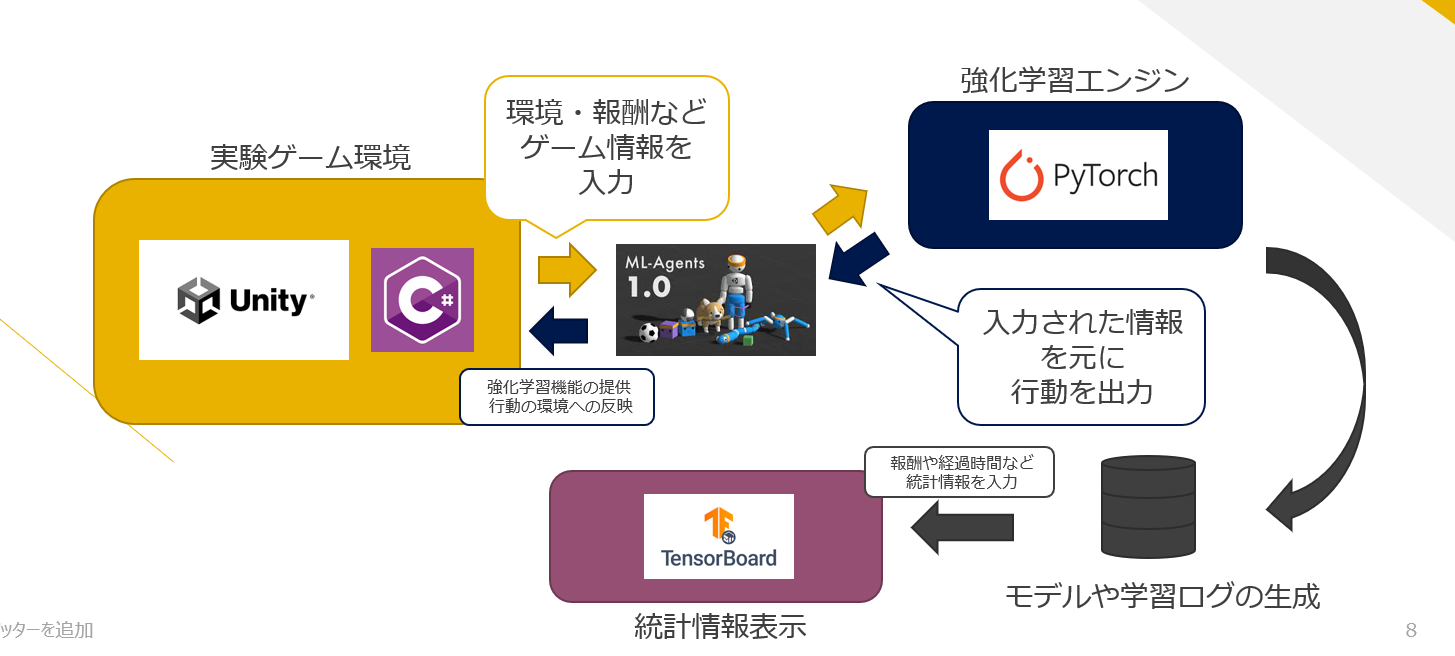
\includegraphics[scale=0.6]{images/system.PNG}
            \caption{作成したアプリの仕様図}
        \end{figure}
        \subsubsection{計算機環境}
        本研究に用いた計算機のスペックは以下の通りである。
        \begin{itemize}
            \item CPU: Intel(R) Core(TM) i7-9700K CPU @ 3.60GHz
            \item GPU: NVIDIA GeForce RTX 2070 8GB
            \item RAM: 32GB
            \item OS: Windows 10 Home 64bit Ver. 21H1
        \end{itemize}
        \subsubsection{ゲーム環境}
        本研究では、以下のようなゲーム環境を用意した。
        \begin{figure}[H]
            \begin{minipage}[b]{0.5\linewidth}
                \centering
                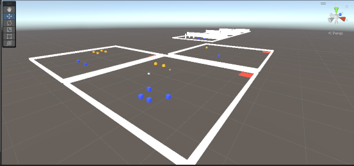
\includegraphics[scale=0.4]{images/flat.png}
                \caption{フラットなフィールド}
            \end{minipage}
            \begin{minipage}[b]{0.5\linewidth}
                \centering
                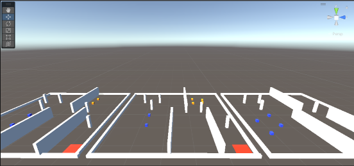
\includegraphics[scale=0.4]{images/shogaibutu.png}
                \caption{障害物を追加したフィールド}
            \end{minipage}
            \begin{minipage}[b]{0.5\linewidth}
                \centering
                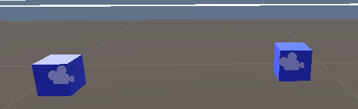
\includegraphics[scale=0.4]{images/Police.png}
                \caption{警察役エージェント}
            \end{minipage}
            \begin{minipage}[b]{0.5\linewidth}
                \centering
                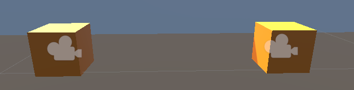
\includegraphics[scale=0.4]{images/Criminer.png}
                \caption{犯人役エージェント}
            \end{minipage}
        \end{figure}
        また、各フィールドの構成は以下の通りである。今回は、スペックの関係上、各チームの人数構成は次の通りとする。
        \begin{itemize}
            \item フラットな環境 : 3個
            \begin{itemize}
                \item 警官1体 vs 犯人1体
                \item 警官4体 vs 犯人2体
                \item 警官2体 vs 犯人4体
            \end{itemize}
            \item 障害物を追加した環境 : 3個
            \begin{itemize}
                \item 警官2体 vs 犯人2体
                \item 警官2体 vs 犯人4体
                \item 警官4体 vs 犯人2体
            \end{itemize}
        \end{itemize}
    \subsection{実験方法}
        \subsubsection{手順}
            本研究では、以下の手順を踏んで実験を行った。
            \begin{enumerate}
                \item Unityで実験環境を作成する。
                \item 警察役AIと犯人役AIの2チームに分かれて実際にドロケーをさせる。
                \item まともにドロケーができるようになるまでの時間を計測する。
                \item 各フィールドにおいて、実際にどのような戦略が行われているのか観察する。
            \end{enumerate}
        \subsubsection{学習アルゴリズムについて}
        本研究では機械学習の中でも強化学習(深層強化学習)に分類される方法で行った。\par 
        \paragraph{強化学習とは} ここで、本研究で使用した強化学習に関して、簡単に説明する。
        
\section{研究結果}
    \subsection{警察側の結果}
    \subsection{逃走側の結果}
\section{考察}
\section{まとめ}
\begin{thebibliography}{99}
    \bibitem{openAI} Bowen Baker, Ingmar Kanitscheider, Todor Markov, Yi Wu, Glenn Powell, Bob McGrew, Igor Mordatch 
    “EMERGENT TOOL USE FROM MULTI-AGENT AUTOCURRICULA ”
    ICLR 2020, 2020-02-11, 28p.


\end{thebibliography}
\section{ソースコード等}
\end{document}